\documentclass[tikz,border=4pt]{standalone}
\usepackage[T1]{fontenc}
\usepackage{newtxtext}
\usetikzlibrary{arrows.meta,positioning,fit,backgrounds}

\definecolor{densitygreen}{HTML}{E3F0E5}
\definecolor{pipelineorange}{HTML}{F8E6D2}
\definecolor{headerblue}{HTML}{DCEAF7}
\definecolor{ink}{HTML}{263746}
\definecolor{linegreen}{HTML}{4F8A5B}
\definecolor{lineorange}{HTML}{C8782D}

\begin{document}
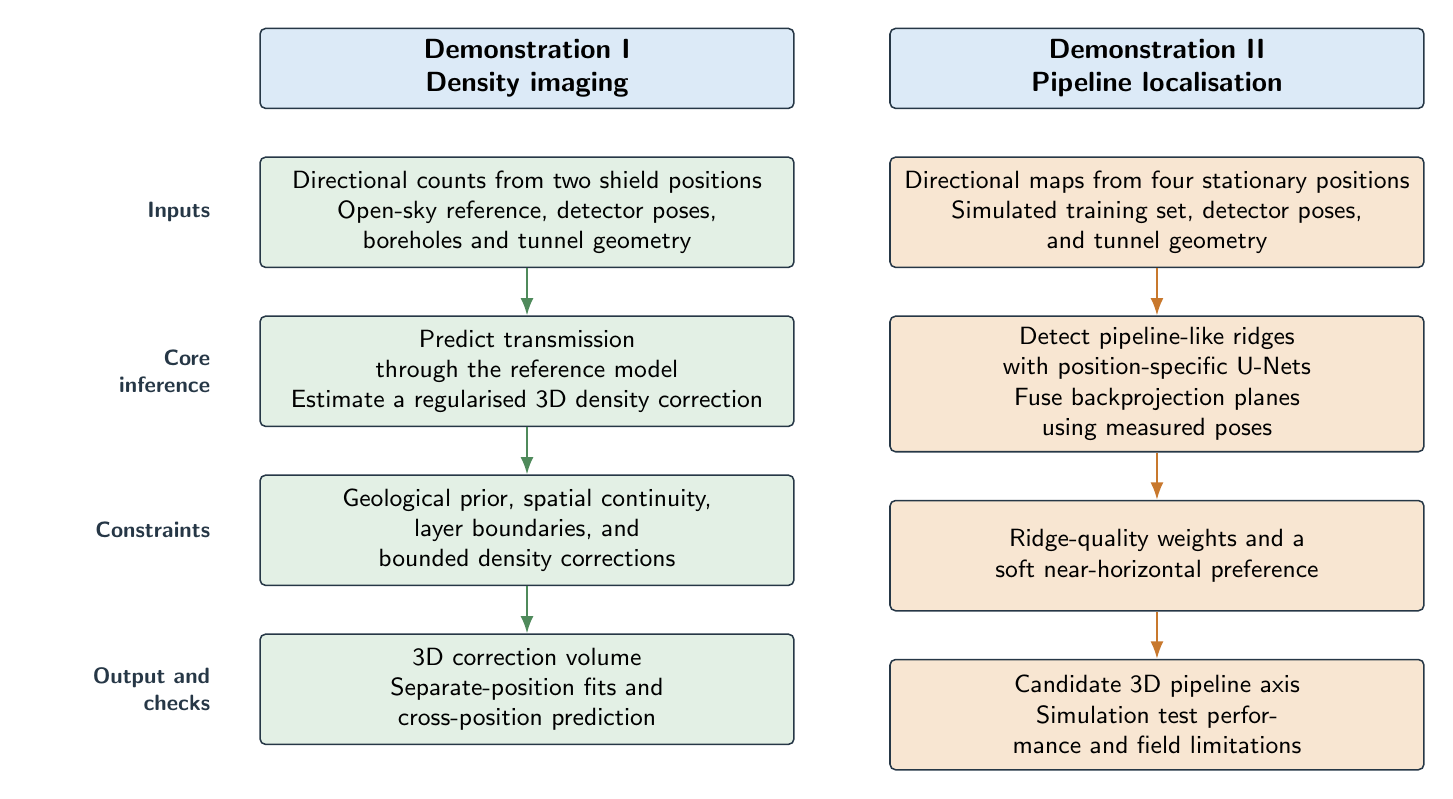
\begin{tikzpicture}[
  font=\sffamily\small,
  >=Latex,
  cell/.style={draw=ink, rounded corners=2pt, line width=0.55pt,
    align=center, text width=65mm, minimum height=14mm, inner sep=4pt},
  density/.style={cell, fill=densitygreen},
  pipeline/.style={cell, fill=pipelineorange},
  head/.style={cell, fill=headerblue, font=\sffamily\bfseries, minimum height=10mm},
  rowlabel/.style={font=\sffamily\bfseries\footnotesize, text=ink,
    align=right, text width=22mm},
  arrow/.style={-{Latex[length=2.2mm]}, line width=0.75pt}
]

\node[head] (dh) {Demonstration I\\Density imaging};
\node[head, right=12mm of dh] (ph) {Demonstration II\\Pipeline localisation};

\node[density, below=6mm of dh] (ddata)
  {Directional counts from two shield positions\\Open-sky reference, detector poses, boreholes and tunnel geometry};
\node[pipeline, below=6mm of ph] (pdata)
  {Directional maps from four stationary positions\\Simulated training set, detector poses,\\and tunnel geometry};

\node[density, below=6mm of ddata] (dmethod)
  {Predict transmission through the reference model\\Estimate a regularised 3D density correction};
\node[pipeline, below=6mm of pdata] (pmethod)
  {Detect pipeline-like ridges with position-specific U-Nets\\Fuse backprojection planes using measured poses};

\node[density, below=6mm of dmethod] (dconstraint)
  {Geological prior, spatial continuity,\\layer boundaries, and bounded density corrections};
\node[pipeline, below=6mm of pmethod] (pconstraint)
  {Ridge-quality weights and a soft near-horizontal preference};

\node[density, below=6mm of dconstraint] (doutput)
  {3D correction volume\\Separate-position fits and cross-position prediction};
\node[pipeline, below=6mm of pconstraint] (poutput)
  {Candidate 3D pipeline axis\\Simulation test performance and field limitations};

\foreach \a/\b in {ddata/dmethod,dmethod/dconstraint,dconstraint/doutput}
  \draw[arrow, draw=linegreen] (\a) -- (\b);
\foreach \a/\b in {pdata/pmethod,pmethod/pconstraint,pconstraint/poutput}
  \draw[arrow, draw=lineorange] (\a) -- (\b);

\node[rowlabel, left=5mm of ddata] {Inputs};
\node[rowlabel, left=5mm of dmethod] {Core\\inference};
\node[rowlabel, left=5mm of dconstraint] {Constraints};
\node[rowlabel, left=5mm of doutput] {Output and\\checks};

\end{tikzpicture}
\end{document}